    \subsection*{What $\lambda$ should we choose?}
    
        There's something we ignored earlier: how do we pick the \textbf{best} value of $\lambda$? We didn't go into detail, but that value of $\lambda$ will affect our algorithm's \textbf{performance}.
        
        This $\lambda$ adjusts exactly how we \textbf{learn}: how much more do we learn \textbf{specifically}, versus \textbf{generally}?
    
        We mentioned that different $\lambda$ values have different \textbf{tradeoffs}, so we need to figure out which $\lambda$ value is best for our problem.
        
        We'll need to \textbf{optimize} our $\lambda$ value! Let's figure out how to go about that.
        
    \subsection*{Tradeoffs: Estimation Error}
    
        High and low $\lambda$ values have benefits and drawbacks. These tradeoffs can be loosely divided into \textbf{two categories}.
        
        When we generalize, we're trying to avoid \vocab{estimation error}: we incorrectly guess the overall distribution we're trying to fit. We \textbf{estimate} poorly if we \textbf{generalize} poorly.\\
        
        \begin{definition}
            \vocab{Estimation error} is the error that results from poorly \gren{estimating} the \purp{solution} we're trying to find. 
            
            This can be caused by \gren{overfitting}, getting a bad (\purp{unrepresentative}) sample, or not having enough \gren{data} to come to conclusion.
        \end{definition}
        
        \miniex Let's try a regression problem, but we'll use only 4 points to make our plot.
        
        \begin{figure}[H]
            \begin{subfigure}
                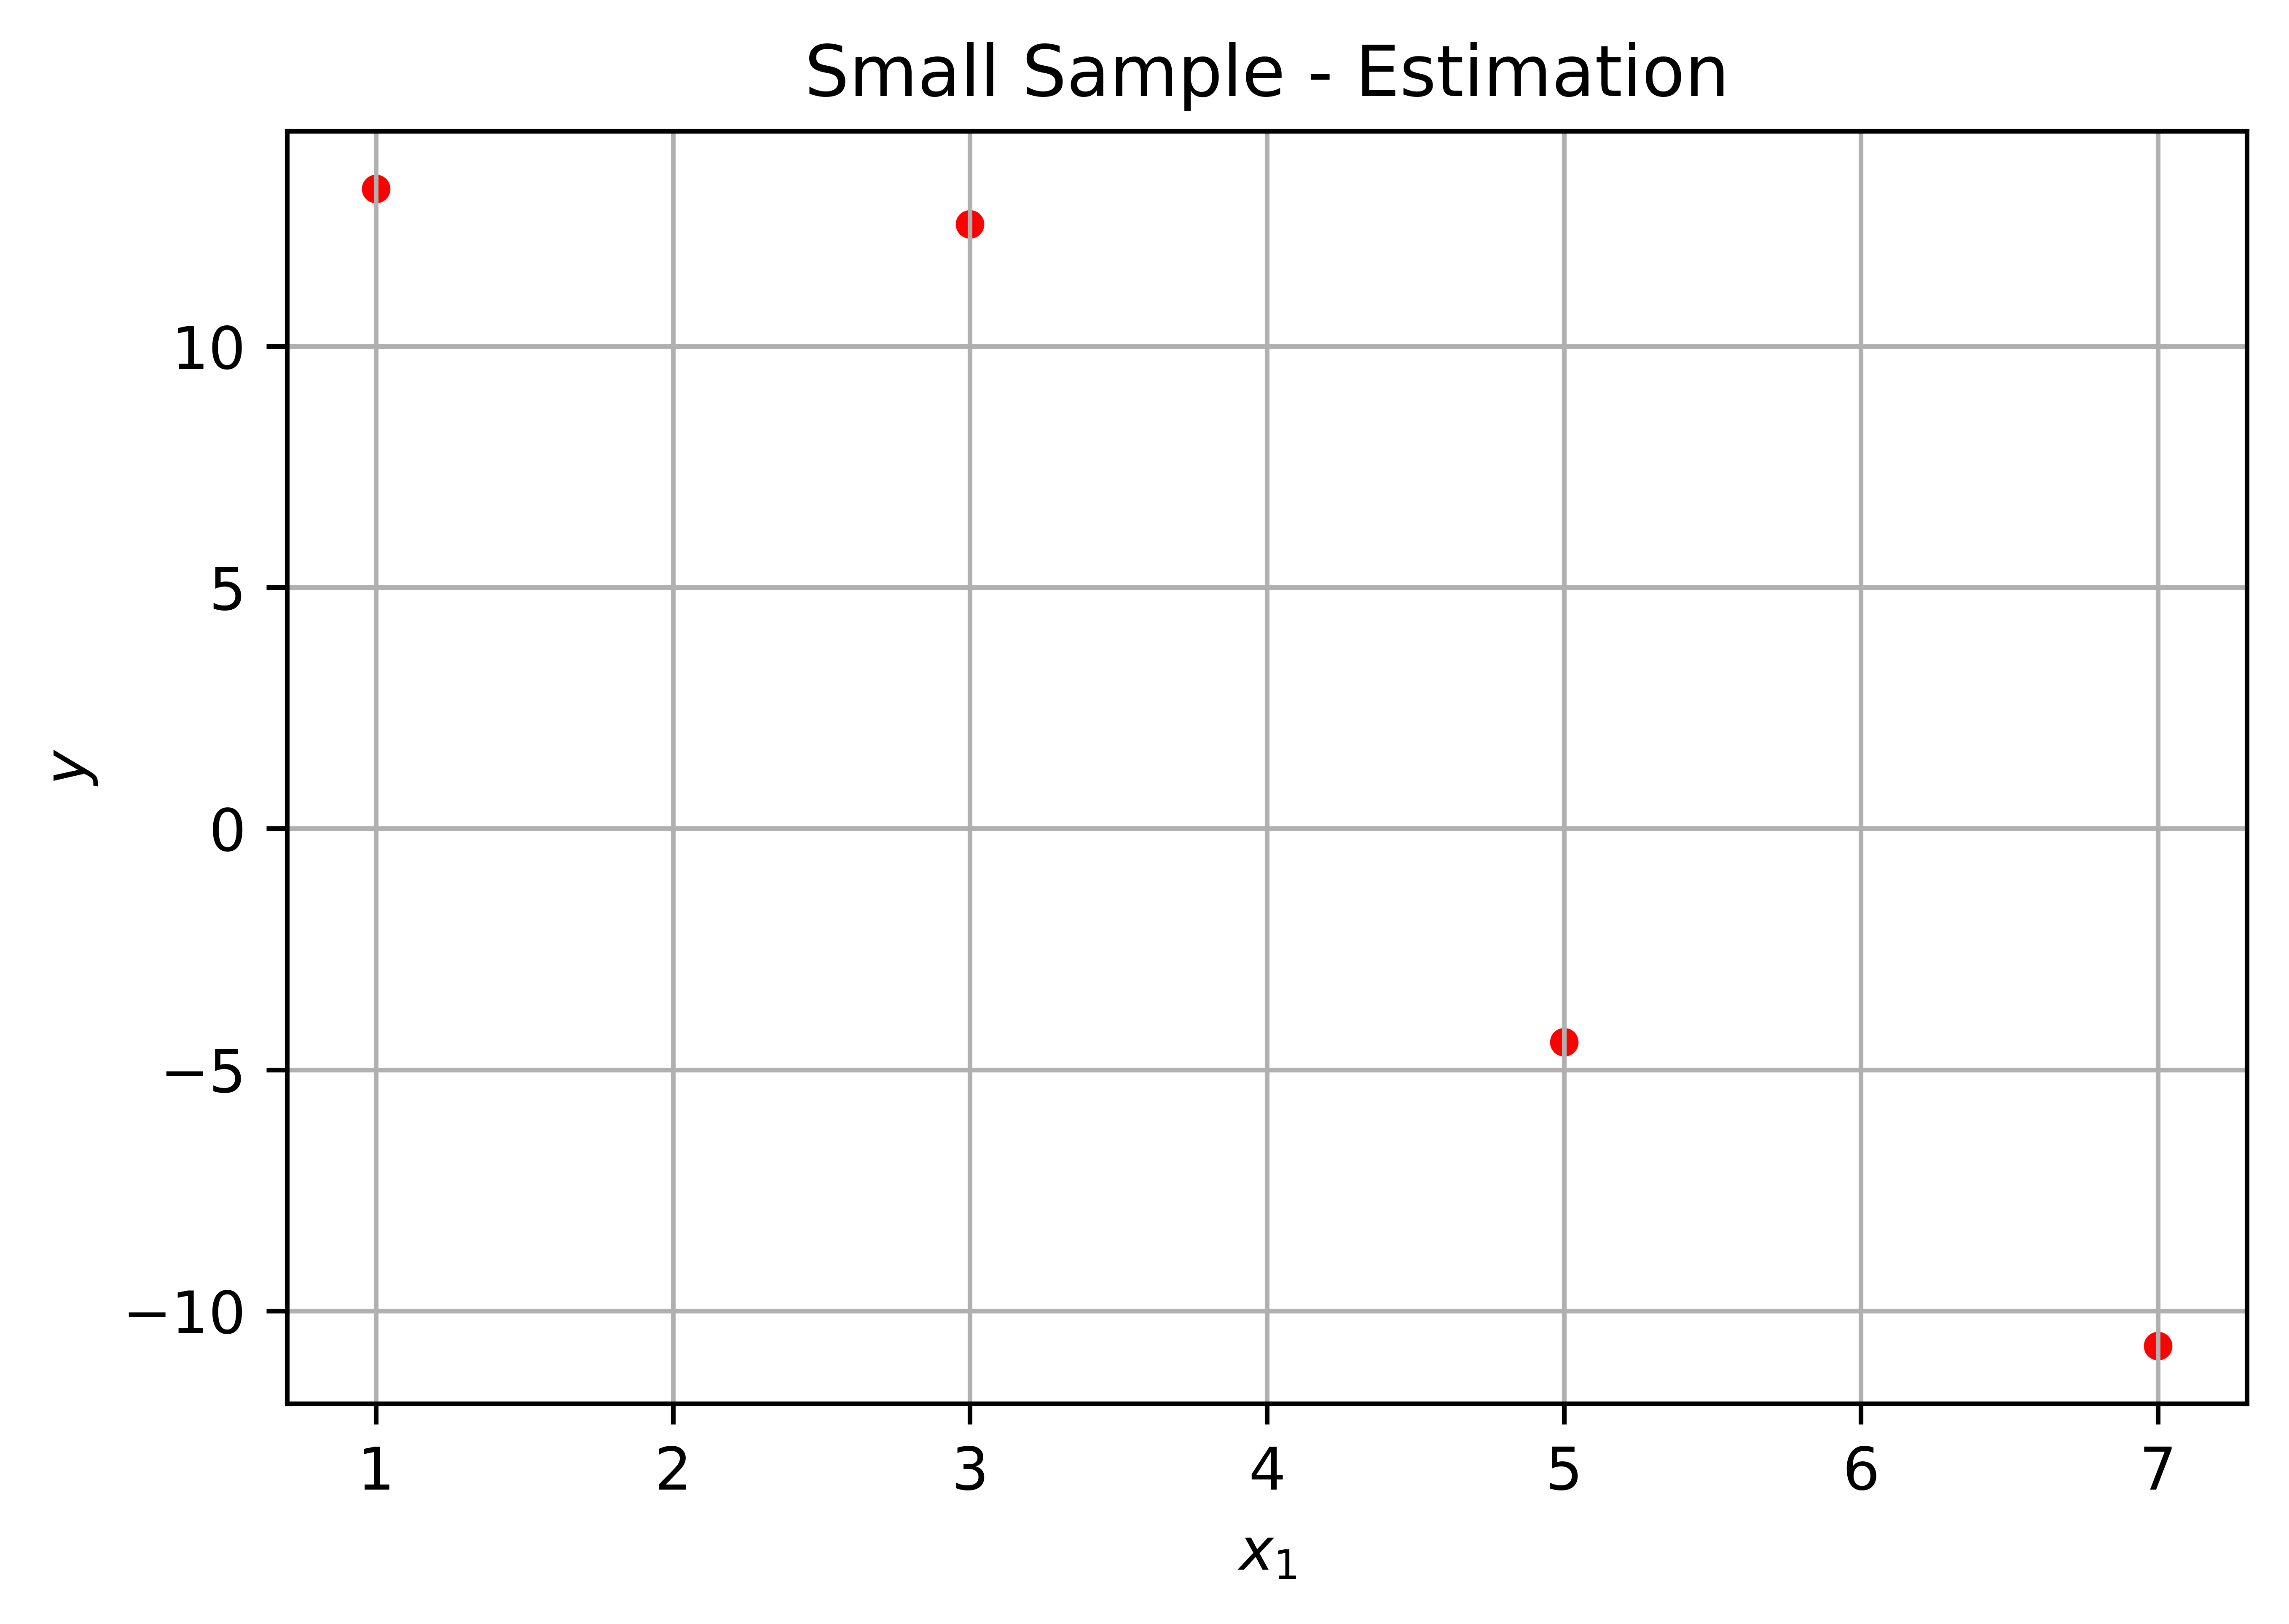
\includegraphics[width=70mm,scale=0.5]{images/regression_images/Estimation_Limited_Sample.png}
            \end{subfigure}
            \begin{subfigure}
                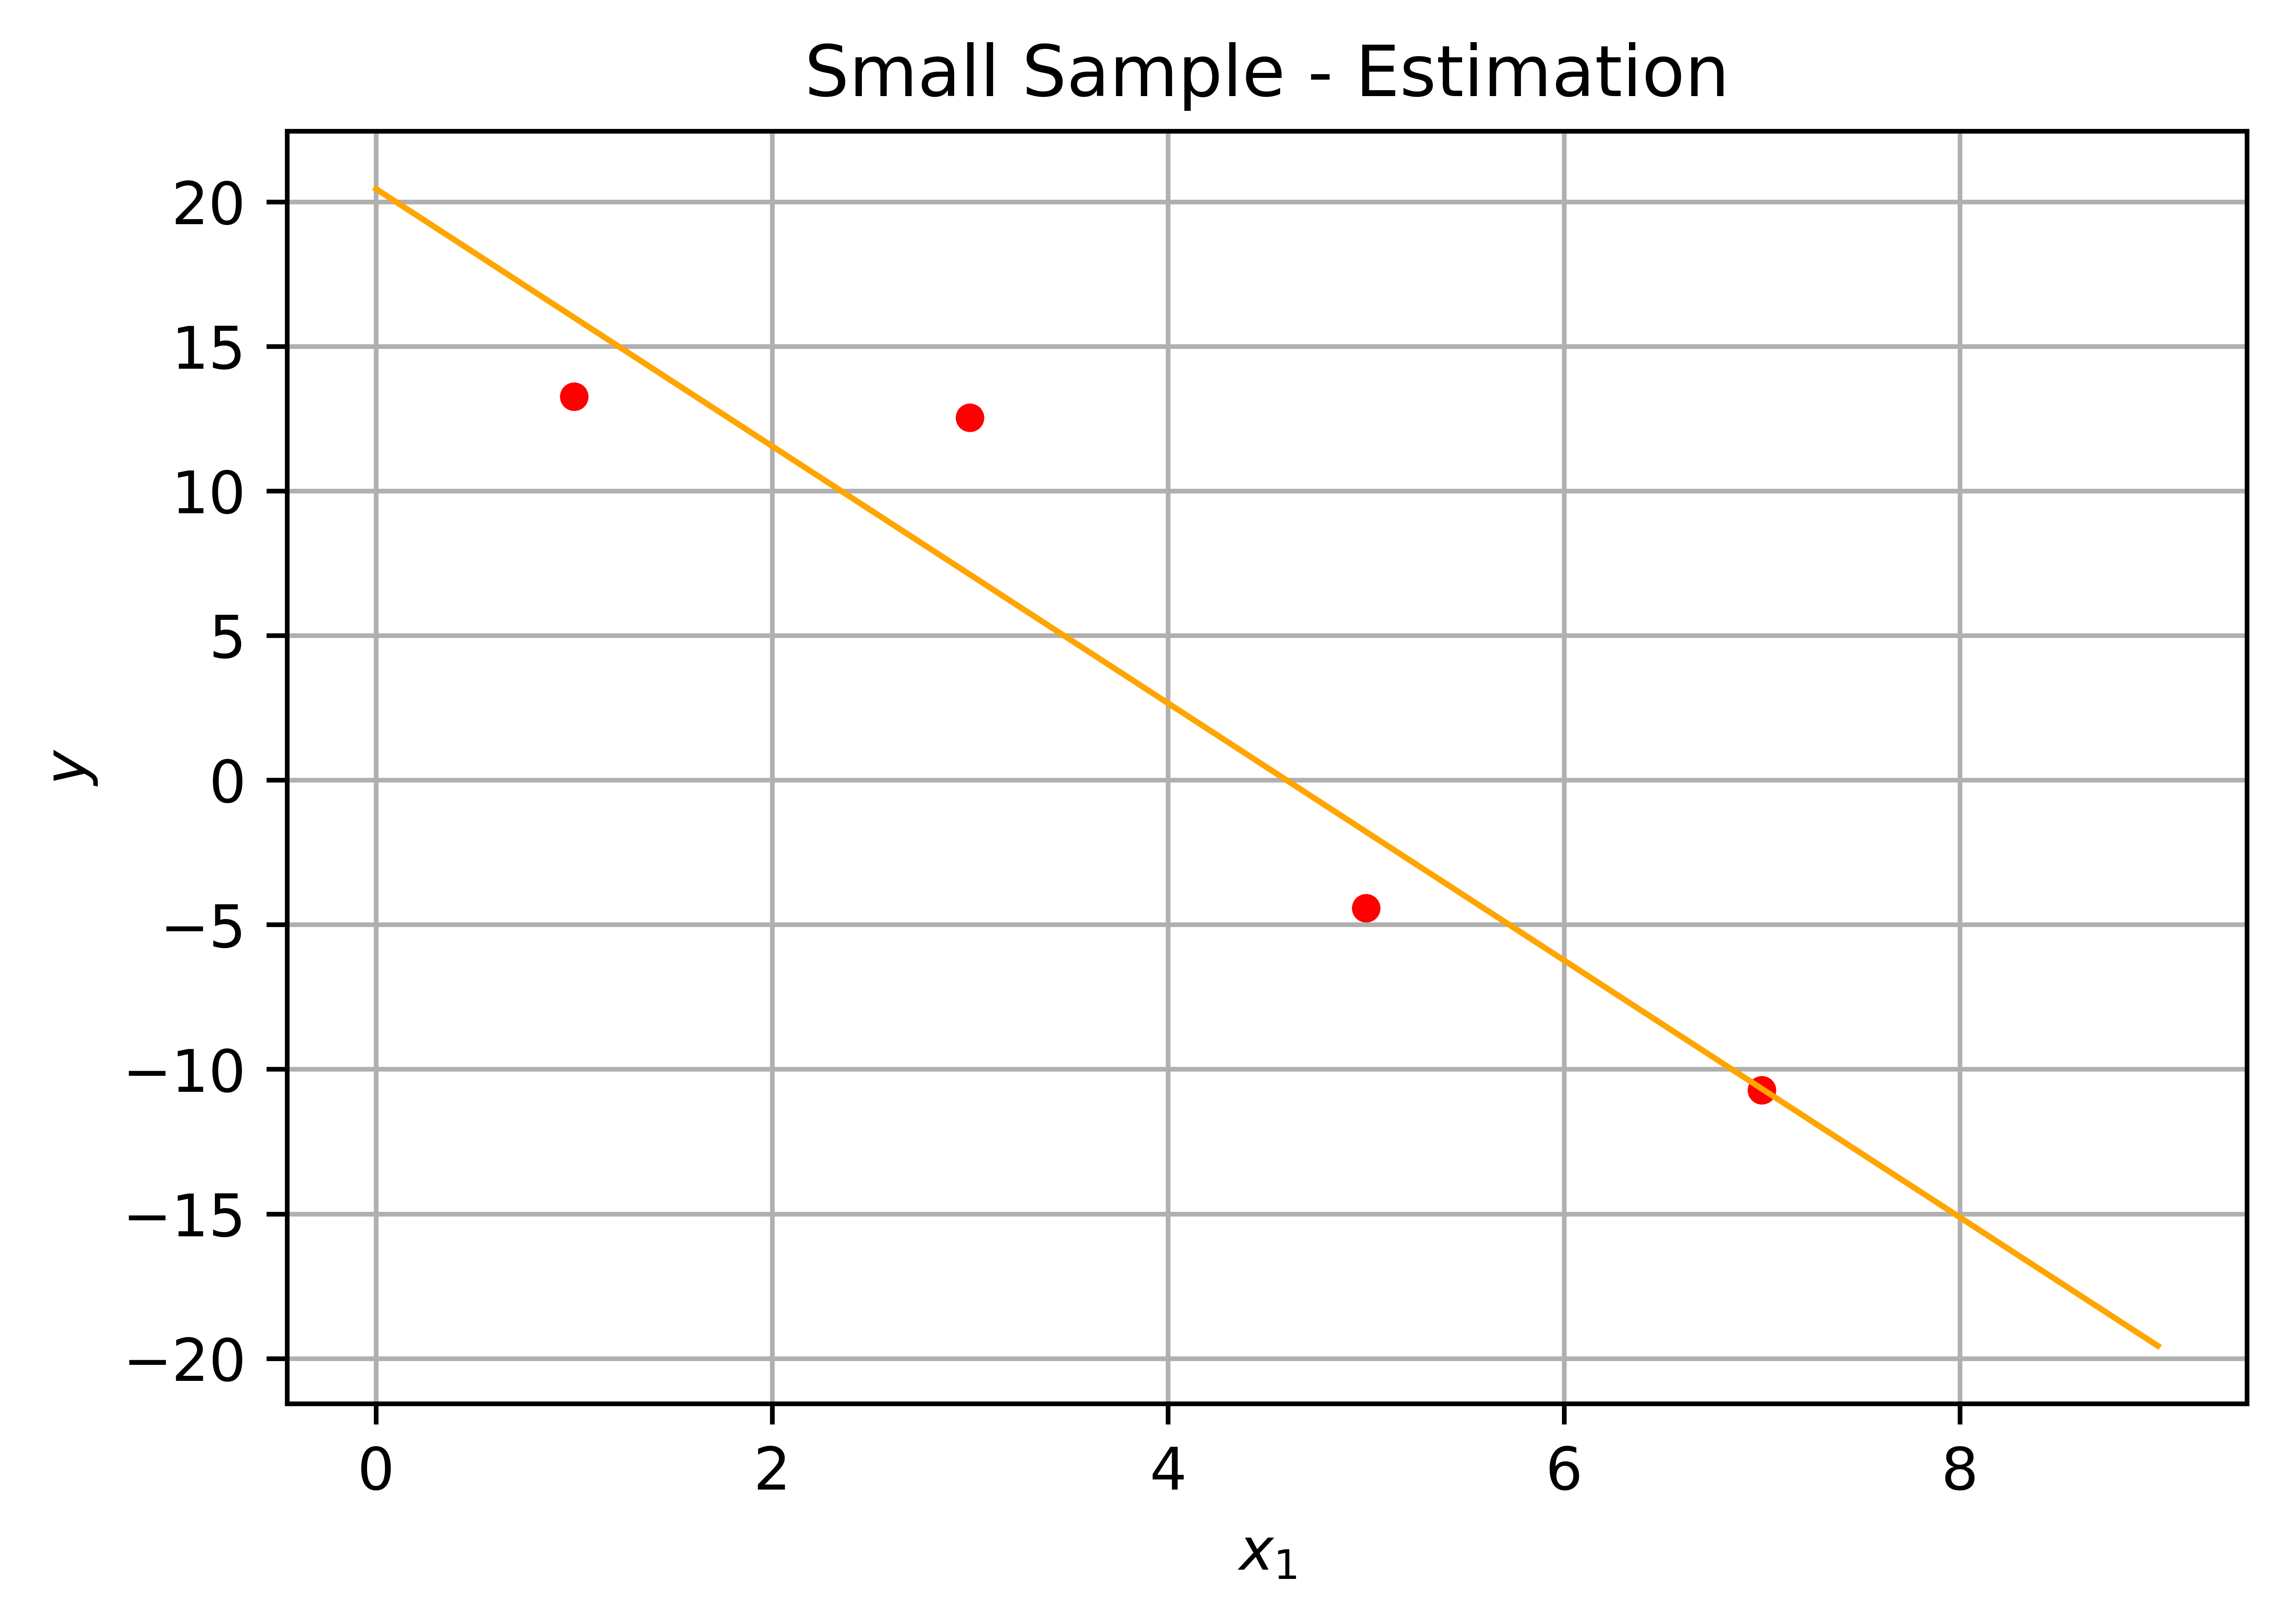
\includegraphics[width=70mm,scale=0.5]{images/regression_images/Estimation_Limited_Sample_Regression.png}
            \end{subfigure}
        
            \caption*{This is the regression solution we get based on our small dataset.}
        \end{figure}
        
        We might be suspicious. One way to reduce \textbf{estimation error} is to increase our number of data points (though this isn't always an option, or sufficient!)
        
        \begin{figure}[H]
            \begin{subfigure}
                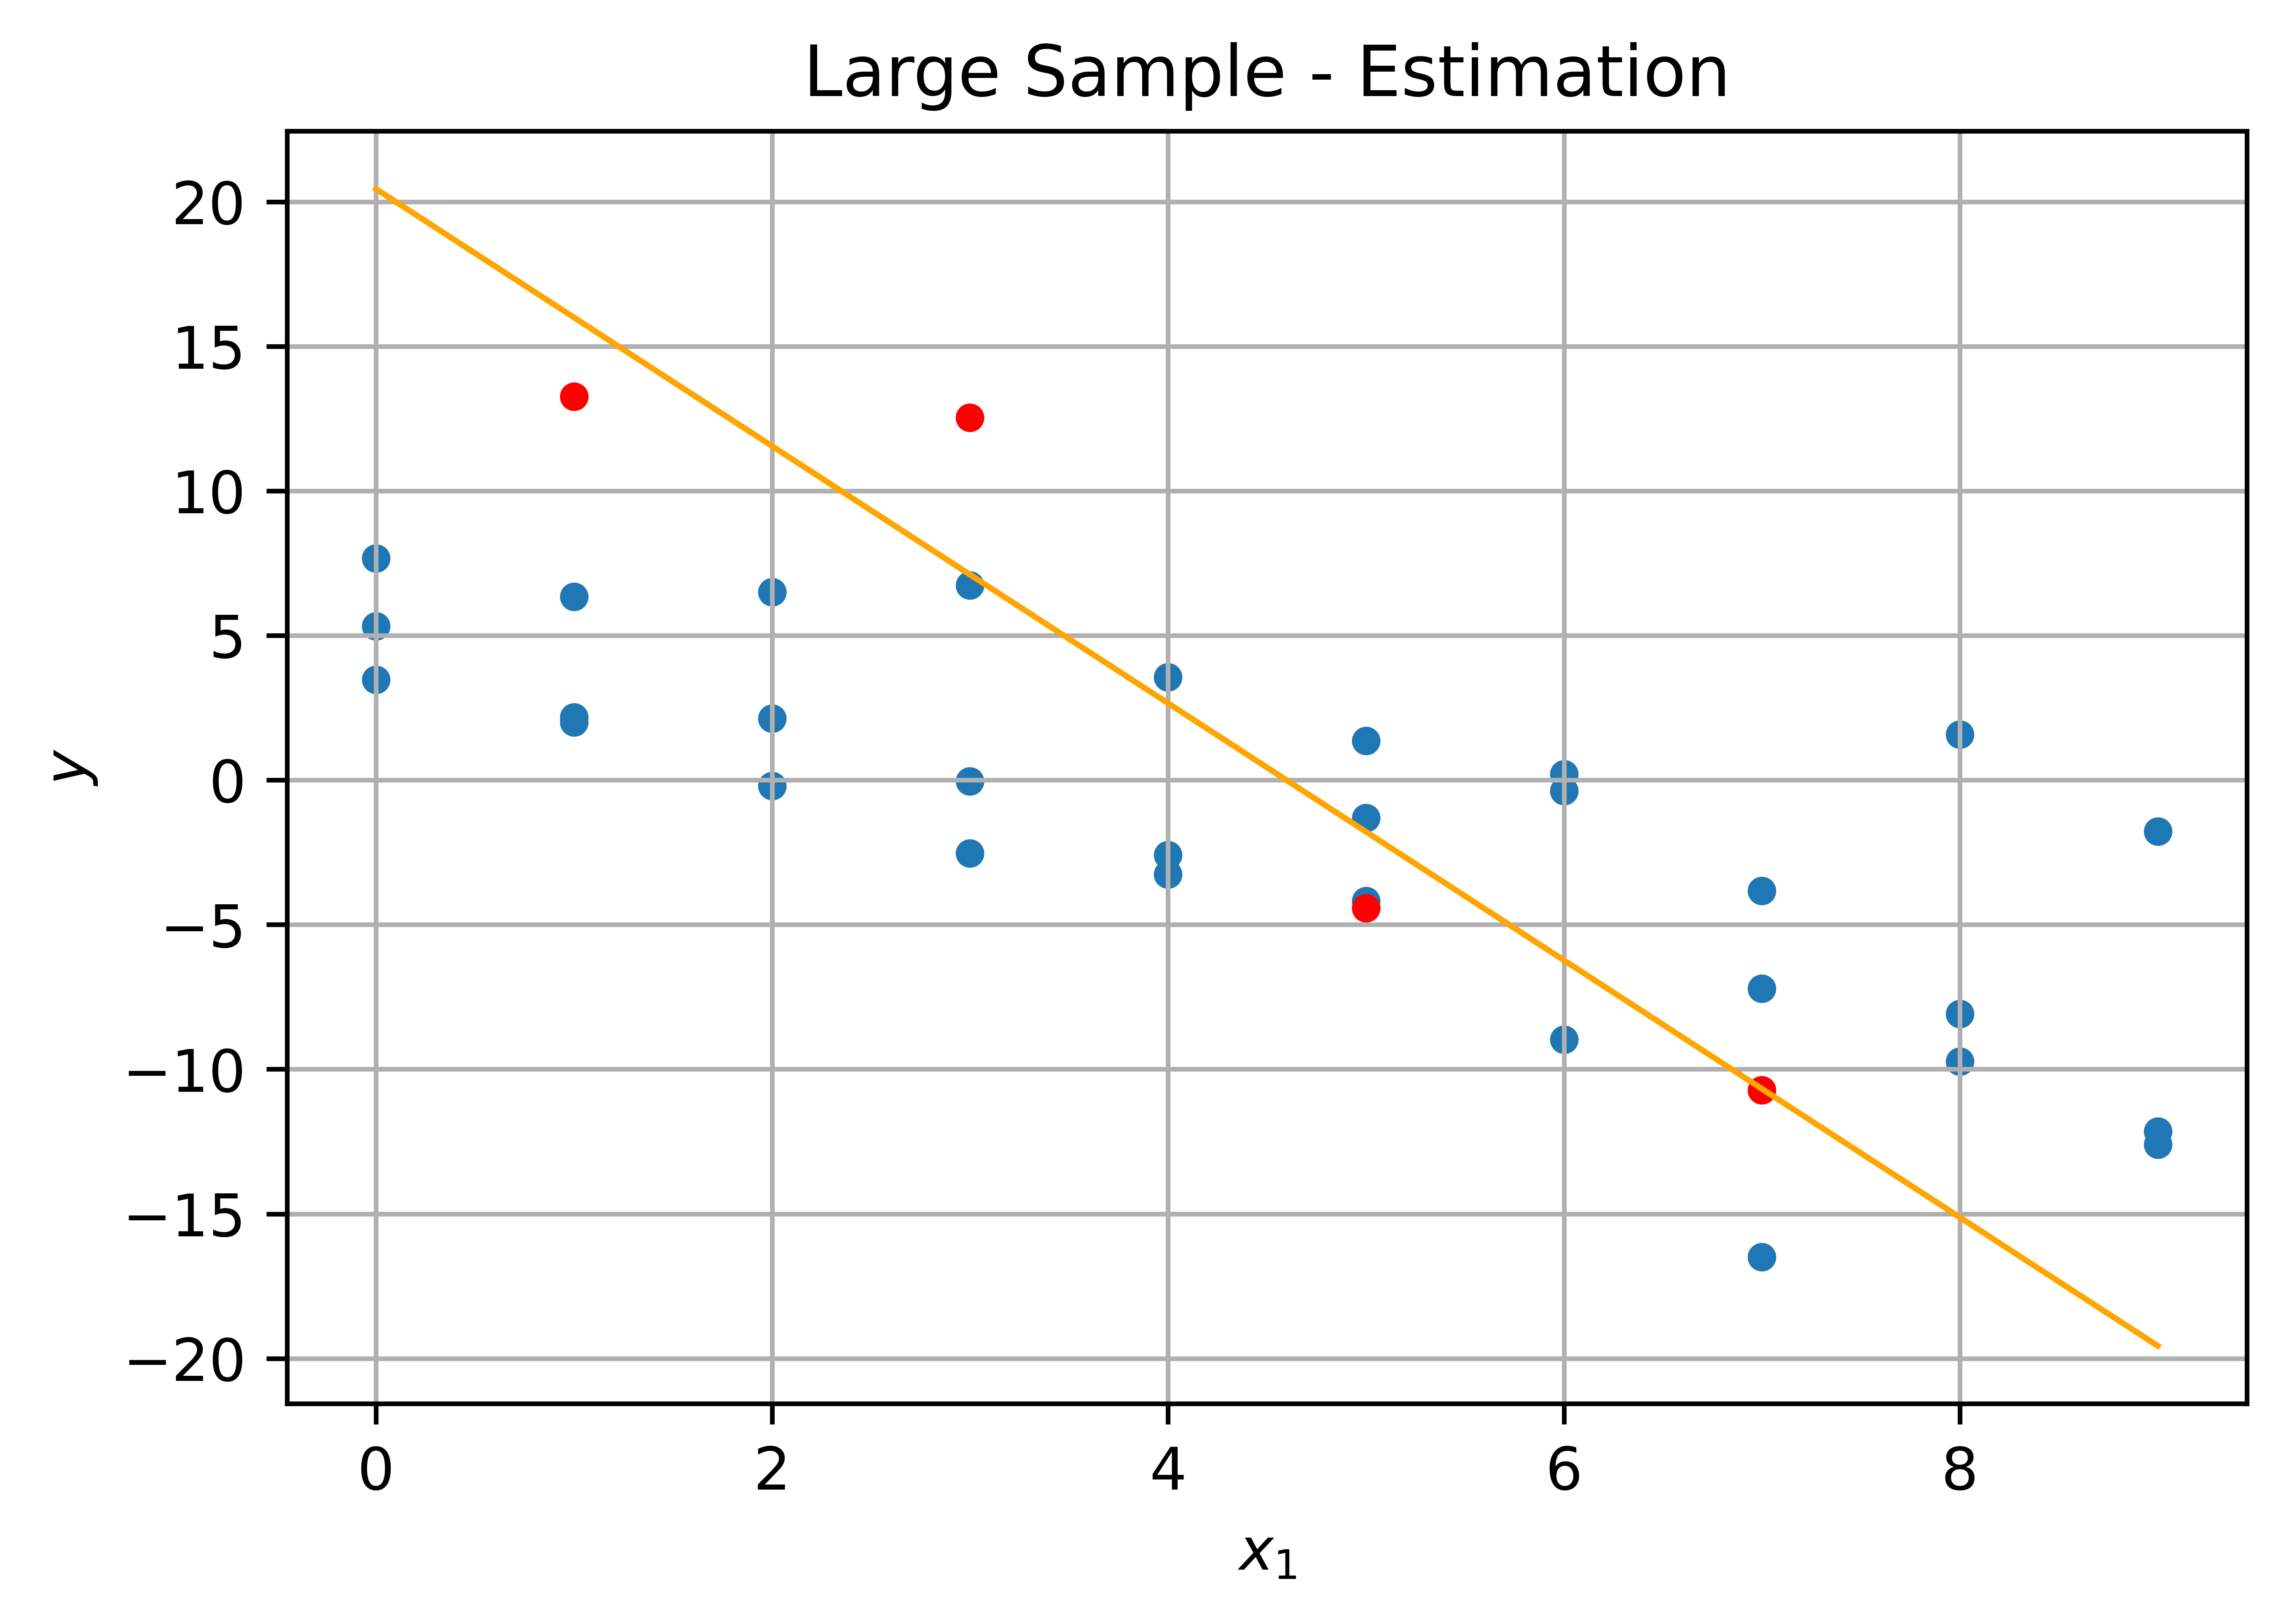
\includegraphics[width=70mm,scale=0.5]{images/regression_images/Estimation_Full_Sample.png}
            \end{subfigure}
            \begin{subfigure}
                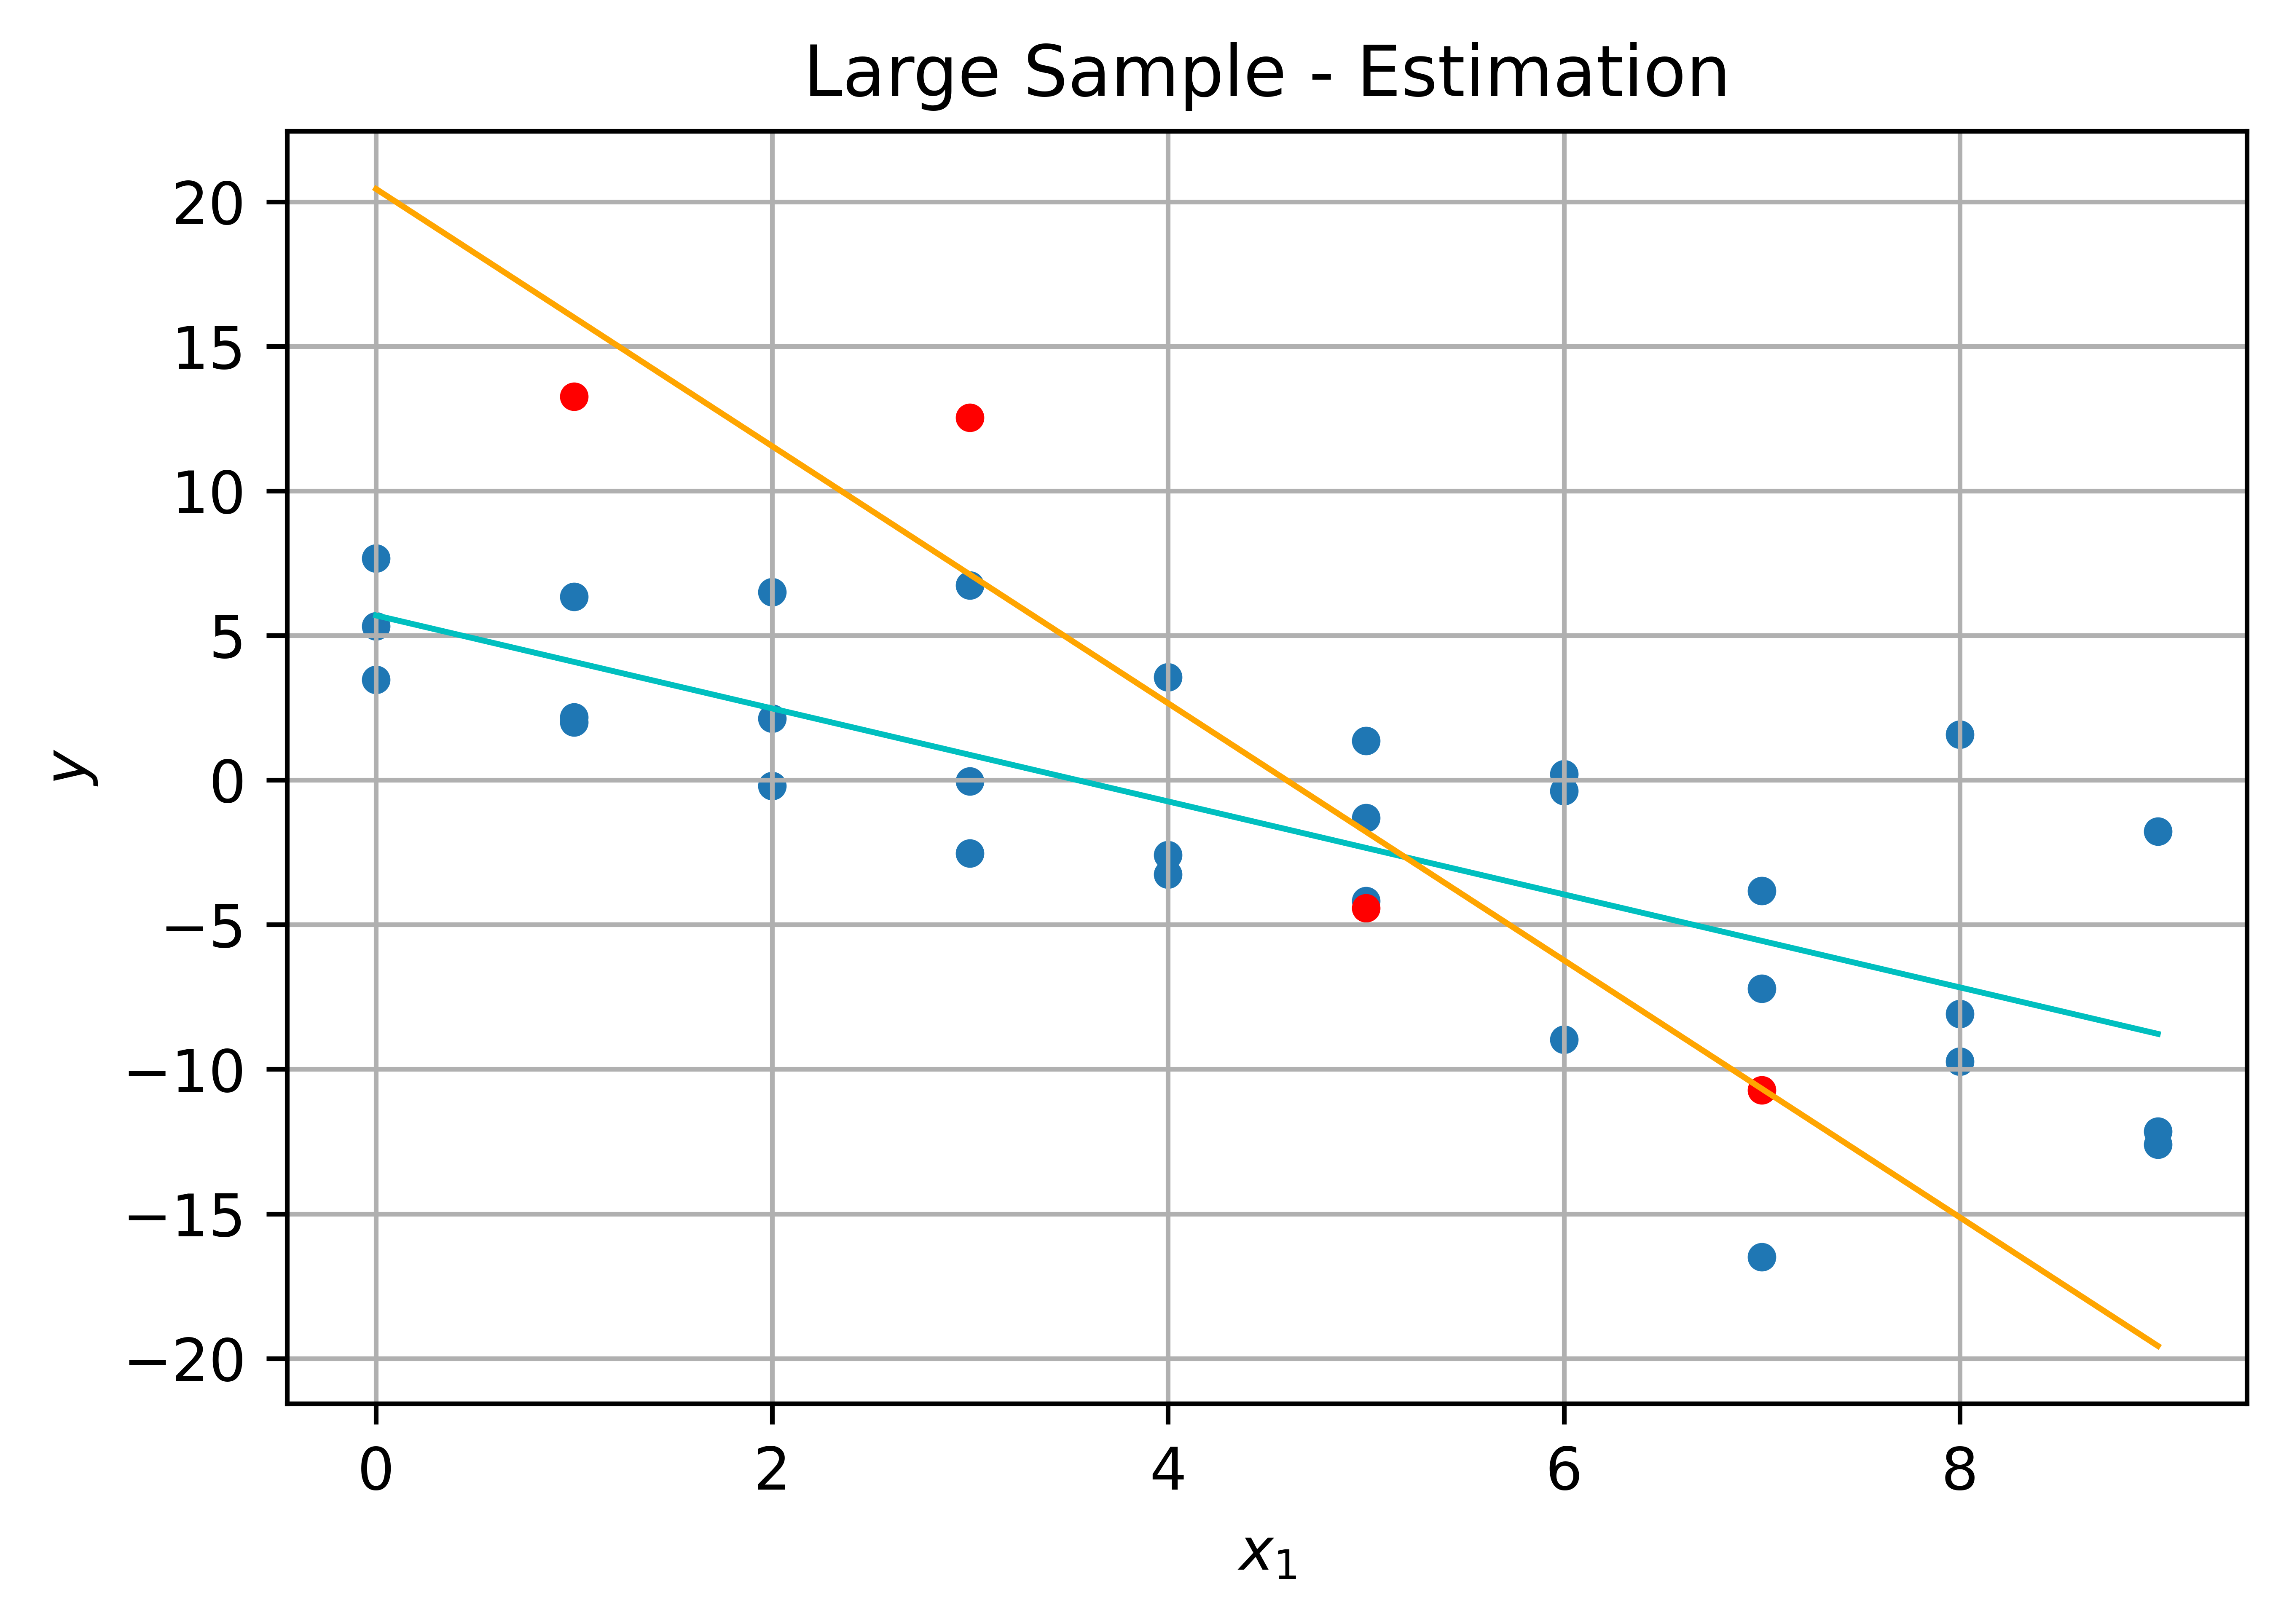
\includegraphics[width=70mm,scale=0.5]{images/regression_images/Estimation_Full_Sample_Regression.png}
            \end{subfigure}
        
            \caption*{Our regression from before doesn't look so good on this model... We make an updated regression, and get a more accurate result.}
        \end{figure}
        
        \begin{clarification}
           $\lambda$ doesn't lower \purp{estimation error} in the \gren{same way} that increasing \purp{sample size} does, but the problem is \gren{similar}.
        \end{clarification}
        
    \subsection*{Tradeoffs: Structural Error}
    
        However, not all problems are caused by estimation error: sometimes, it \textbf{isn't even possible} to get a good result - you chose the wrong \textbf{model class}.
        
        This means the \textbf{structure} of your model is the problem, not your method of \textbf{estimation}. Thus, we call this \vocab{structural error}.\\
        
        \begin{definition}
            \vocab{Structural error} is the error that results from having the wrong \gren{structure} for the \purp{task} you are trying to accomplish.
            
            This can result from the \gren{wrong class} of model, but sometimes, your model class doesn't have the \purp{expressiveness} it needs for a complex problem.
            
            It can also happen if your algorithm \purp{limits} the available models in some way, like how $\lambda$ does.
        \end{definition}
        
        \miniex If the \textbf{true shape} of a distribution is a parabola $x^2$, there is \textbf{no} linear function $mx+b$ that can match that: this creates \textbf{structural error}.
        
        \begin{figure}[H]
            \begin{subfigure}
                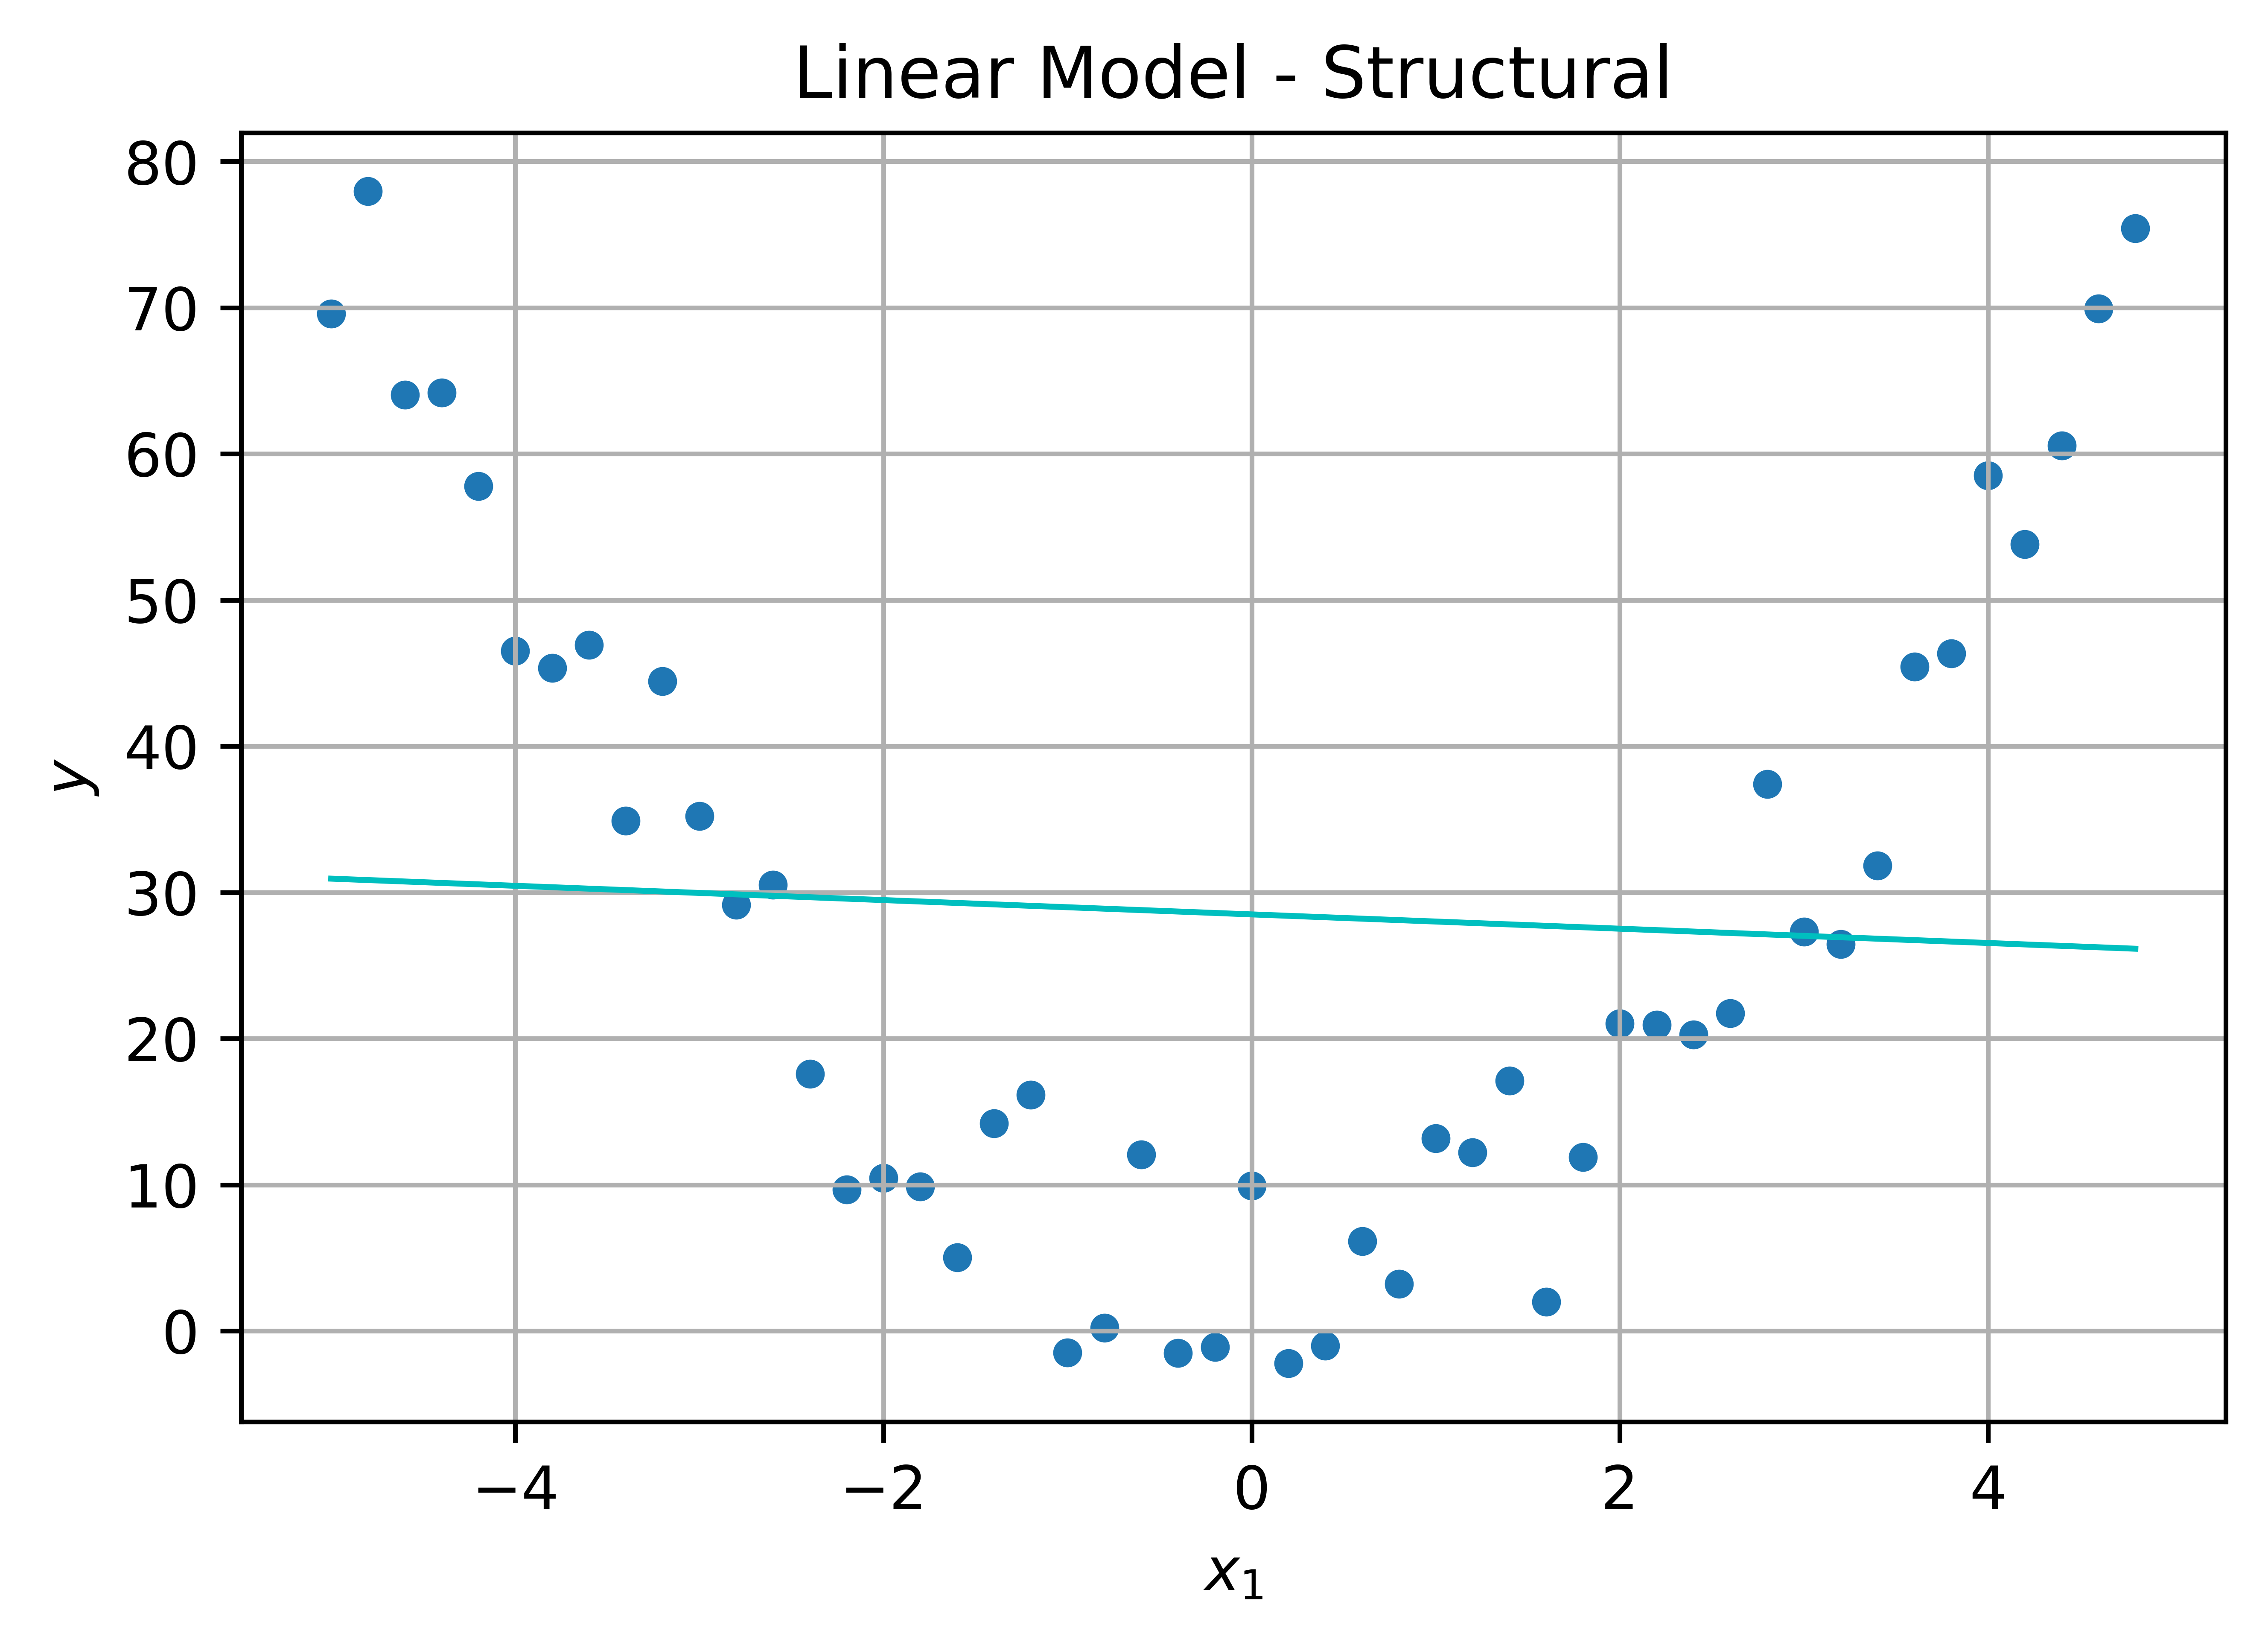
\includegraphics[width=70mm,scale=0.5]{images/regression_images/Structural_Linear_Model.png}
            \end{subfigure}
            \begin{subfigure}
                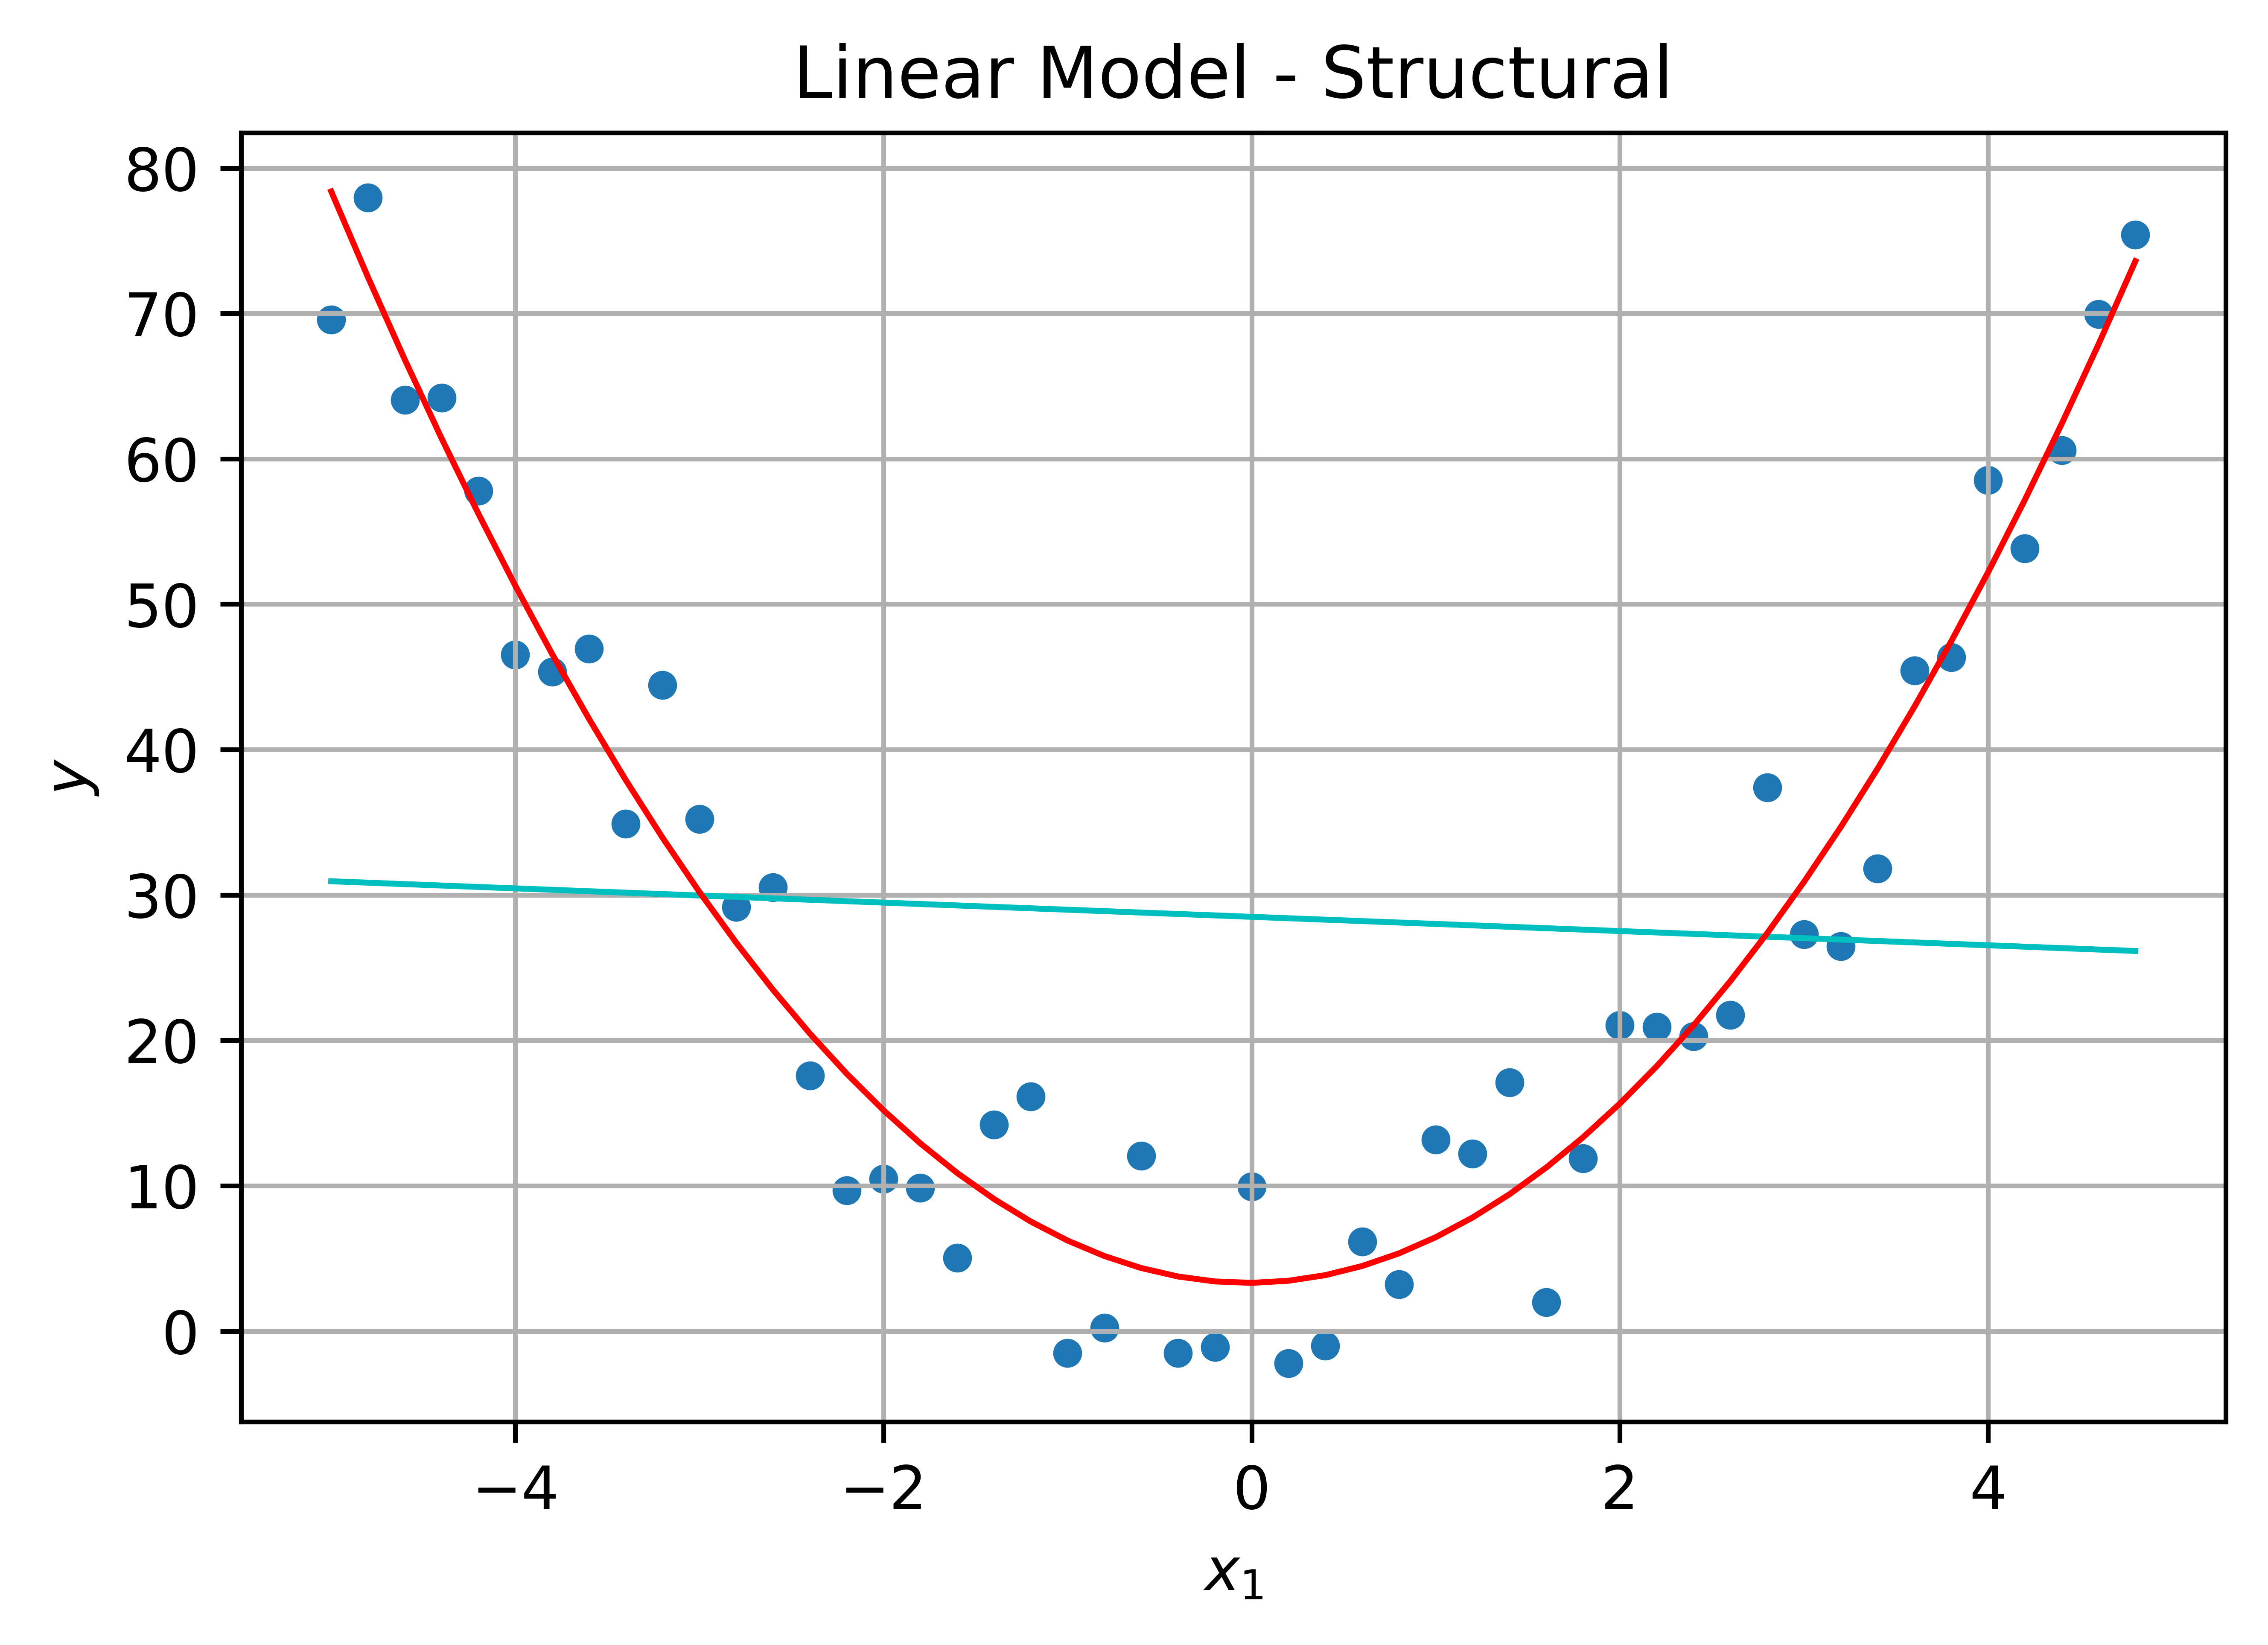
\includegraphics[width=70mm,scale=0.5]{images/regression_images/Structural_Quad_Model.png}
            \end{subfigure}
        
            \caption*{Our \textbf{linear} model isn't able to represent a quadratic function... so, we switch to a more \textbf{expressive} model: a \textbf{quadratic} equation.}
        \end{figure}
        
        \note{Remember that \textbf{expressiveness} is about how many possible models you have: if you have more models, you can solve more problems.}
        
        \begin{clarification}
           Note that $\lambda$ does not restrict our model class \purp{as severely} as \gren{switching polynomial order}, like above. 
        
            But, $\lambda$ \purp{limits} the use of larger $\theta$, which does make it \gren{unable} to solve some problems. So, the \purp{structural error} problem is similar.
        \end{clarification}
        
    \subsection*{Tradeoffs of $\lambda$}
        
        Based on these two categories, we can discuss the tradeoffs of $\lambda$ more easily.
        
        As we mentioned, regularization \textbf{reduces} estimation error: 
        
        If we overfit to our current data, we are poorly \textbf{estimating} the distribution, because the training data may not perfectly \textbf{represent} it.\\
        
        \begin{concept}
            A \vocab{large $\lambda$} means \purp{more regularization}: we more strongly push for a more \gren{general} model, over a more \gren{specific} one.
            
            This results in...
            
            \begin{itemize}
                \item \gren{Reduced} estimation error
                \item \purp{Increased} structural error
            \end{itemize}
        \end{concept}
        
        However, \textbf{regularization} also \textbf{limits} the possible models we can use - those it views as less "general", it \textbf{penalizes}.
        
        That means the scope of possible models is \textbf{smaller} - some models are no longer \textbf{acceptable}. What if the only valid solution was in that space we \textbf{restricted}? Well, then we can't \textbf{find} it.
        
        That means there are certain \textbf{structural} limits on our model: that means that regularization \textbf{increases} structural error!\\
        
        \begin{concept}
            A \vocab{small $\lambda$} means \purp{less regularization}: we care less about a more \gren{general} model, allowing more \gren{specific} data to come into play.
            
            This results in...
            
            \begin{itemize}
                \item \purp{Increased} estimation error
                \item  \gren{Reduced} structural error
            \end{itemize}
        \end{concept}